\chapter{肌肉结构和动力学} \label{chap:chap5}


如果你想理解功能,那就研究结构。

\begin{flushright}
	——弗朗西斯$\cdot$克里克
\end{flushright}


\begin{figure}[!htb]
	\centering
	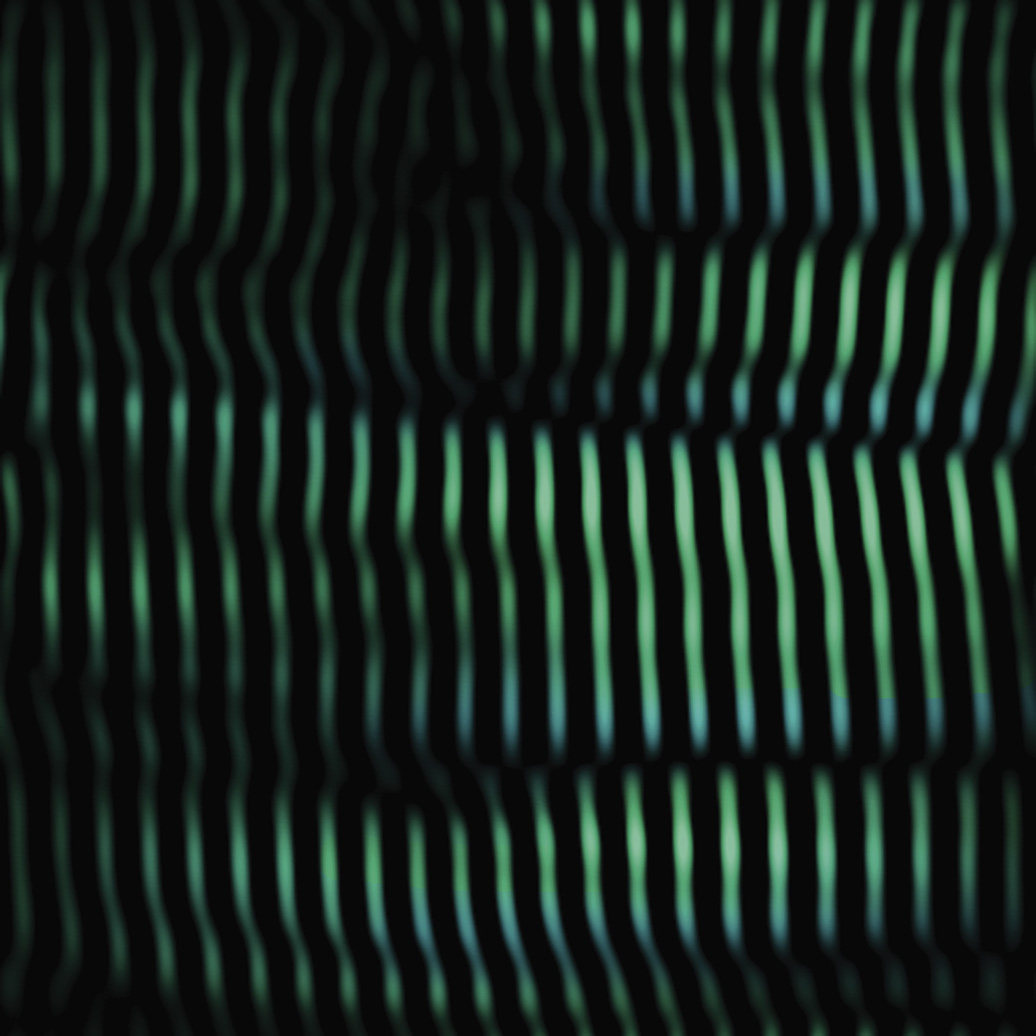
\includegraphics[width=1.0\linewidth]{chap4/4_0}
	% 加星号(*)表示不加编号
	\caption*{ \label{fig:5_0}}
\end{figure}


为了理解人类和动物的运动,研究人员开展了各种各样的实验。
生物力学家通过测量数千人的关节运动、地面反作用力和肌电信号来研究全身运动。
生理学家研究了单个肌肉,以表征肌肉激活和力量产生的动态。
肌肉驱动模拟使我们能够将这两个领域联系起来,将全身运动的生物力学测量与针对单个肌肉进行的实验相结合。
我们将在第~\ref{chap:chap10}~至~\ref{chap:chap12}~章中看到,肌肉驱动模拟可以深入了解肌肉在产生运动中的作用,并提供一些在人体运动时几乎无法测量的重要量的估计值,例如肌肉产生的力量和它消耗的能量。


肌肉动力学建模对于创建肌肉驱动的运动模拟至关重要。
然而,一刀切的模型并不适用,因为每块肌肉都有其独特的结构来适应其独特的功能。
例如,一些肌肉负责手指的精细运动控制,而另一些肌肉则在运动过程中支撑身体重量(图~\ref{fig:5_1})。
所有骨骼肌都具有肌节的层级排列,但肌肉在几个重要方面存在差异。
这些差异包括它们的大小和结构,以及肌肉纤维的几何排列。
因此,肌肉的计算模型必须捕捉所有肌肉共同的肌肉力量产生特征,同时还要能够表征每块肌肉的独特特征。


\begin{figure}[!htb]
	\centering
	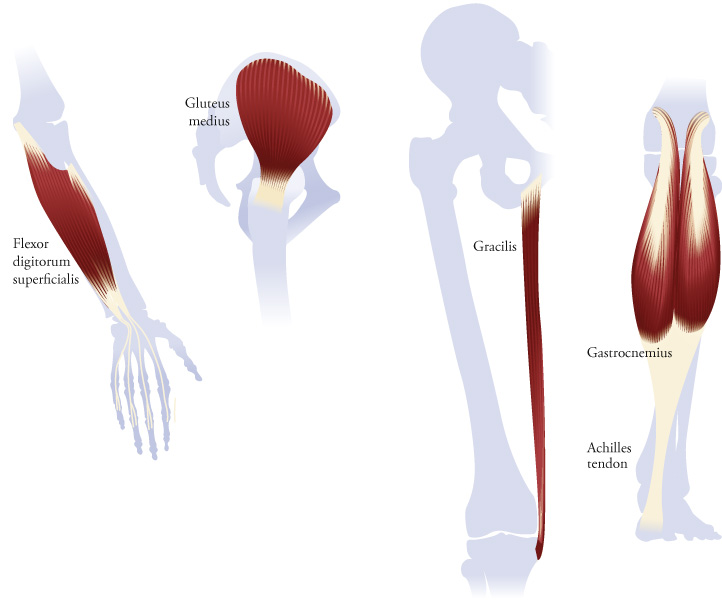
\includegraphics[width=1.0\linewidth]{chap5/5_1}
	\caption{全身肌肉的结构和功能各不相同。
		浅屈指肌(最左侧)通过四条肌腱控制手指屈曲;
		宽阔的臀中肌和纤细的股薄肌产生髋关节外展和内收力矩;
		腓肠肌(最右侧)通过较长的跟腱止于跟骨。 \label{fig:5_1}}
\end{figure}


在本章中,我们将了解如何创建一个通用的肌肉力量产生模型,以及如何对其进行定制以代表身体中的几乎任何肌肉。
我们将要描述的肌肉模型属于以 A. V. Hill 命名的一类模型,除了我们在第~\ref{chap:chap4}~章中看到的“推我拉你”实验之外,他还进行了许多肌肉的基础研究。
我的博士生导师 Felix Zajac 改进了 Hill 型模型,并将其带入了现代计算机模拟时代\cite{zajac1989muscle}。
具体来说,Zajac 开发了一个仅包含四条通用曲线和五个肌肉特定参数的模型,所有这些参数都可以从实验数据中得出并用于调整模型。
Zajac 模型的简单性对于涉及数十块肌肉的动态模拟至关重要,但它足够详细,可以表示不同大小、强度和结构的肌肉的动态。


图~\ref{fig:4_18}~总结了所有肌肉共同的肌肉力量产生特征。
这些特征包括 3 条曲线,描述肌肉长度与其产生的力之间的非线性关系:主动力-长度曲线、被动力-长度曲线和力-速度曲线。
由于肌肉通过肌腱附着在骨骼上,我们还必须考虑这种结缔组织的特性,我们用肌腱的力-长度曲线来描述它。
我们使用 5 个参数缩放这些通用曲线以表示特定的肌肉:
(1)最佳肌纤维长度 $l_o^M$;
(2)最佳纤维长度下的肌纤维羽状角 $\phi_o$ ;
(3)最大等长肌肉力量,$F_o^M$;
(4)最大肌肉收缩速度 $v_\text{max}^M$;
和(5)肌腱松弛长度,$l_s^T$。
本章首先介绍这 5 个特定于肌肉的参数。
我们将了解每个参数如何影响肌肉力量,并将其纳入肌肉-肌腱动力学模型中。


\section{最佳肌纤维长度$l_o^M$}

正如我们在第~\ref{chap:chap4}~章中看到的,肌节能够产生的主动力取决于其长度(图~\ref{fig:4_6})。
肌节能够产生最大等长收缩力的长度称为其最佳长度。
由于肌纤维由多个($n$)个首尾相连的肌节组成,因此肌纤维也存在一个最佳长度($l_o^M$),当其每个组成肌节都达到其最佳长度($l_o^S$)时,肌纤维便会达到该最佳长度:
%
\begin{equation}
	l_o^M = n l_o^S \label{eq:5_1}
\end{equation}

公式~\ref{eq:5_1}~假设肌纤维上串联的所有肌节长度相同。
肌肉在运动过程中会伸长和缩短,这会影响肌节粗肌丝和细肌丝相互滑动时产生的主动力。
最佳长度较长的肌纤维(即串联肌节较多)具有更宽的主动力-长度曲线,并且可以在更宽的长度范围内产生其最大主动力的很大一部分(图~\ref{fig:5_2},顶部)。
增加肌纤维的最佳长度也会增加其最大缩短速度():

\begin{figure}[!htb]
	\centering
	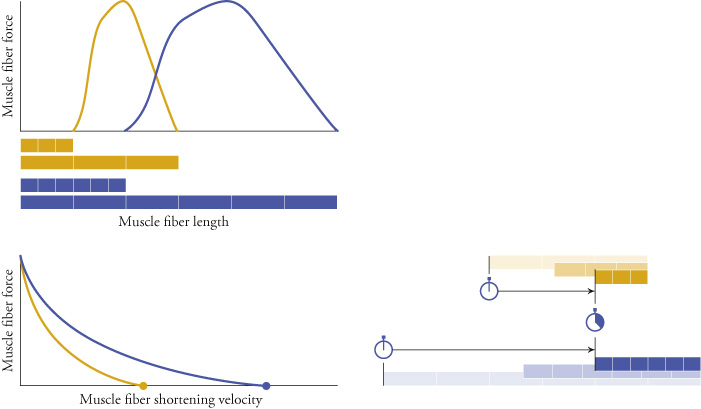
\includegraphics[width=1.0\linewidth]{chap5/5_2}
	\caption{最佳肌纤维长度较长的肌肉,其主动力-长度曲线(上图)更宽,最大缩短速度也更高(下图)。
		请注意,长肌纤维(蓝色)的示意图中,肌节数量是短肌纤维(橙色)的两倍,因此长肌纤维在给定时间内可以缩短 2 倍的距离(右下图)。 \label{fig:5_2}}
\end{figure}

\begin{equation}
	v_{\text{max}}^M = n v_{\text{max}}^S \label{eq:5_2}
\end{equation}
%
其中,$v_\text{max}^S$表示肌节的最大缩短速度。
因此,随着肌肉最佳纤维长度的增加,力-速度曲线也会变宽(图~\ref{fig:5_2},底部)。


生物肌肉由长度不同的肌束构成,肌束本身包含长度也不同的纤维,这些纤维甚至可能终止于肌束内。
然而,在我们的模型中,我们假设肌肉中的所有纤维长度相同——许多(但并非所有)肌肉-肌腱动力学模型都做出了这一假设。
我们进一步假设所有纤维都是直的、平行的且共面的。
因此,为了表征肌肉的力-长度和力-速度特性,我们只是放大了肌纤维的相应特性,而这些特性仅仅是肌节相同特性的放大版本。



\section{最佳纤维长度下的肌纤维羽状角$\phi_o$}

肌肉通常通过肌腱附着于骨骼。
在平行纤维肌腱中,例如缝匠肌,其纤维沿着肌腱方向排列(图~\ref{fig:5_3})。
在大多数其他肌肉中,例如股直肌,其纤维与肌腱呈锐角排列;我们称这些肌肉为羽状肌。
“羽状肌”一词源于拉丁语,意为“羽毛状”,而羽状肌的结构确实让人联想到鸟类的羽毛。

\begin{figure}[!htb]
	\centering
	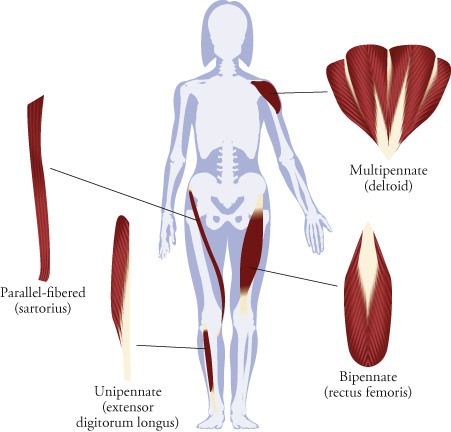
\includegraphics[width=0.8\linewidth]{chap5/5_3}
	\caption{具有不同结构的肌肉的例子:
		平行纤维肌肉、单羽状肌肉、双羽状肌肉和多羽状肌肉。 \label{fig:5_3}}
\end{figure}

如果所有肌纤维都附着在肌腱的一侧,我们称该肌肉为单羽状肌;如果肌纤维附着在肌腱的两侧,则称该肌肉为双羽状肌。
在多羽状肌中,肌腱分支和肌纤维结构可能很复杂。
因此,我们假设给定肌肉中的所有纤维都以相同的角度(称为羽状角 ($\phi$))附着于肌腱,并采用图~\ref{fig:5_4}~所示的肌肉-肌腱几何模型。
由此,我们得到肌纤维中的力 ($F^M$) 和肌腱中的力 ($F^T$) 之间的以下关系:

\begin{figure}[!htb]
	\centering
	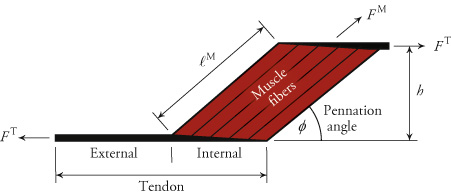
\includegraphics[width=0.75\linewidth]{chap5/5_4}
	\caption{肌纤维和肌腱的简化几何表示。
		肌纤维被假设为直的、平行的、共面的、等长的,并以相同的羽状角 ($\phi$) 附着于肌腱。
			当肌纤维缩短或伸长,羽状角增大或减小时,平行四边形的高度 $h$(以及面积)保持不变\cite{zajac1989muscle}。 \label{fig:5_4}}
\end{figure}

\begin{equation}
	F^T = F^M cos(\phi) 
	\label{eq:5_3}
\end{equation}

现在,参考图~\ref{fig:5_4},我们可以解释生物肌肉如何在纤维长度发生变化的情况下保持体积恒定。
随着图中纤维的缩短,想象一下它们以这样的方式缩短,使得图~\ref{fig:5_4}中的平行四边形保持相同的高度 $h$。
平行四边形的顶部将保持不变,但底部将被向右拉,平行四边形将变得更接近矩形。
然而,只要高度保持不变,面积也将保持不变,这符合平行四边形面积等于其底边和高乘积的几何规则。
我们以二维方式绘制了该图,但三维运动类似,并确保肌肉的体积不变。
简而言之,羽状肌不是通过膨胀来维持体积,而是通过剪切来维持体积。


在上述过程中,羽状角不断增大,从纤维传递到肌腱的力不断减小,直到纤维与肌腱垂直,图中的肌肉呈矩形(即$\phi$ = 90度)。
我们使用参数$\phi_o$表示肌纤维达到最佳长度时的羽状角(即$l^M = l_o^M$)。
我们所描述的固定高度近似法可能会对收缩时明显隆起的肌肉引入误差,但它为研究肌肉结构的功能含义提供了一个简单的几何模型。


除了公式~\ref{eq:5_3}~中表达的关系外,羽状肌在决定肌肉的产力能力方面也起着至关重要的作用。
一般来说,羽状肌角度越大,在给定体积内能够容纳的肌肉纤维越多。
想象一下在矩形房间铺设硬木地板的类似情况:可以使用相对较少的长木板来延伸房间的长度,或者使用大量较短的木板以对角线方向铺设。
同样,与相同体积的平行纤维肌肉相比,羽状肌的纤维更短,因此主动力-长度曲线和力-速度曲线更窄(图~\ref{fig:5_2})。
当然,羽状肌也包含更多的纤维,其后果将在下一节探讨。



\section{最大等长肌肉力量$F_o^M$}

我们 5 个肌肉参数系列中的第三个参数相对容易理解,但测量起来却不那么容易。
这就是最大等长肌肉力。
它被定义为肌肉在最大程度激活并保持最佳纤维长度时产生的力量。


对于活体人体来说,最大等长肌力很难测量,因为我们无法将一块肌肉与其他肌肉分离,并只对该肌肉施加阻力。
因此,我们使用一个称为生理横截面积(PCSA;图~\ref{fig:5_5})的指标。
这是肌肉垂直于纤维方向的横截面积。
需要注意的是,在羽状肌中,该横截面积与肌肉的纵轴倾斜。
最大等长肌力可以通过以下方式估算:

\begin{figure}[!htb]
	\centering
	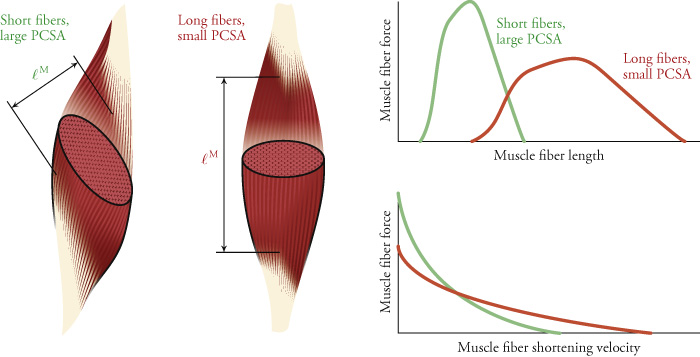
\includegraphics[width=1.0\linewidth]{chap5/5_5}
	\caption{左图所示的肌肉体积相同,但PCSA(主成分分析面积)、最佳纤维长度和羽状角不同。
		羽状肌越多,产生的主动力越大,但纤维越短;
		因此,其主动力-长度曲线和动力-速度曲线更高,但更窄\cite{lieber2002skeletal}。 \label{fig:5_5}}
\end{figure}

\begin{equation}
	F_o^M = \text{PCSA} \sigma_o^M
	\label{eq:5_4}
\end{equation}
%
其中 $\sigma_o^M$ 是肌肉的比张力(也称为峰值等长应力),即单位面积可产生的最大肌肉力。
在构建健康肌肉模型时,该参数的典型值为 $\sigma_o^M = 0.3 \; \text{MPa}$ 。


在上一节中,我们注意到,羽状肌的纤维比相同体积的平行纤维肌更短,但数量也更多。
因此,尽管羽状肌的力-长度和力-速度曲线较窄,但这些曲线也会更高,因为羽状肌的PCSA(以及因此产生的最大等长力)更大(图~\ref{fig:5_5})。


肌肉纤维的长度和收缩速度不仅仅受其几何形状的影响,我们将在接下来的两节中看到这一点。
尽管如此,我们已经可以观察到肌肉的结构如何影响其所能执行的功能范围:
在其他条件相同的情况下,羽状肌能够比相同体积的平行纤维肌产生更大的力量,但其长度范围较小,收缩速度也较低。


